% ============================================================
%  Projet Réussite - Dossier d'Analyse
%  Auteur : Matthieu PELINGRE
%  M2SDD - Universite de Lorraine - 2025-2026
% ============================================================
\documentclass[12pt, a4paper, french]{report}

% ----------------------------------------------------------------
% Encodage et langue
% ----------------------------------------------------------------
\usepackage[utf8]{inputenc}
\usepackage[T1]{fontenc}
\usepackage[french]{babel}
\usepackage{lmodern}
\usepackage{microtype}

% ----------------------------------------------------------------
% Mise en page
% ----------------------------------------------------------------
\usepackage{geometry}
\geometry{
  top=2.5cm, bottom=2.5cm,
  left=2.8cm, right=2.8cm,
  headheight=15pt
}

% ----------------------------------------------------------------
% Couleurs (palette Python)
% ----------------------------------------------------------------
\usepackage{xcolor}
\definecolor{pythonblue}{HTML}{356D9C}
\definecolor{pythonyellow}{HTML}{FED03E}
\definecolor{pythondark}{HTML}{1E4068}
\definecolor{pythonlight}{HTML}{D6E8F5}
\definecolor{codeblue}{HTML}{3572A5}
\definecolor{codebg}{HTML}{F5F9FC}
\definecolor{codegreen}{HTML}{336633}
\definecolor{codegray}{HTML}{777777}
\definecolor{alertred}{HTML}{CC3333}
\definecolor{alertbg}{HTML}{FFF0F0}

% ----------------------------------------------------------------
% En-tetes et pieds de page
% ----------------------------------------------------------------
\usepackage{fancyhdr}
\pagestyle{fancy}
\fancyhf{}
\fancyhead[L]{\small\color{pythonblue}\textit{Projet Réussite -- Dossier d'Analyse}}
\fancyhead[R]{\small\color{pythonblue}\textit{M2SDD -- 2025-2026}}
\fancyfoot[C]{\small\thepage}
\renewcommand{\headrulewidth}{0.4pt}

% ----------------------------------------------------------------
% Titres
% ----------------------------------------------------------------
\usepackage{titlesec}
\titleformat{\chapter}[display]
  {\normalfont\huge\bfseries\color{pythondark}}
  {\color{pythonblue}\large\chaptertitlename\ \thechapter}
  {8pt}
  {\Huge\color{pythondark}}
  [\vspace{4pt}\color{pythonyellow}\rule{\textwidth}{2pt}]
\titlespacing*{\chapter}{0pt}{-10pt}{24pt}

\titleformat{\section}{\large\bfseries\color{pythonblue}}{\thesection}{1em}{}
\titleformat{\subsection}{\normalsize\bfseries\color{pythondark}}{\thesubsection}{1em}{}
\titleformat{\subsubsection}{\normalsize\itshape\color{pythonblue}}{\thesubsubsection}{1em}{}

% ----------------------------------------------------------------
% Graphiques, figures, tableaux
% ----------------------------------------------------------------
\usepackage{graphicx}
\usepackage{float}
\usepackage{caption}
\usepackage{subcaption}
\usepackage{booktabs}
\usepackage{array}
\usepackage{multirow}
\captionsetup{font=small, labelfont={bf,color=pythonblue}}

% ----------------------------------------------------------------
% Listings
% ----------------------------------------------------------------
\usepackage{listings}
\lstdefinestyle{python}{
  language=Python,
  basicstyle=\small\ttfamily,
  keywordstyle=\color{codeblue}\bfseries,
  stringstyle=\color{codegreen},
  commentstyle=\color{codegray}\itshape,
  numberstyle=\tiny\color{codegray},
  numbers=left, stepnumber=1, numbersep=6pt,
  breaklines=true, frame=single,
  rulecolor=\color{pythonblue!30},
  backgroundcolor=\color{codebg},
  tabsize=4, showstringspaces=false,
  captionpos=b
}
\lstset{style=python}

% ----------------------------------------------------------------
% Boites colorees
% ----------------------------------------------------------------
\usepackage{tcolorbox}
\tcbuselibrary{skins, breakable}

\newtcolorbox{notebox}{
  colback=pythonlight, colframe=pythonblue,
  fonttitle=\bfseries, title={Remarque},
  arc=4pt, boxrule=1pt
}

\newtcolorbox{analysebox}[1]{
  colback=pythonlight, colframe=pythonblue,
  coltitle=white, fonttitle=\bfseries,
  title={#1}, arc=4pt, boxrule=1pt
}

\newtcolorbox{warningbox}[1][Attention]{
  colback=alertbg, colframe=alertred,
  coltitle=white, fonttitle=\bfseries,
  title={#1}, arc=4pt, boxrule=1pt
}

\newtcolorbox{resultbox}[1]{
  colback=pythonyellow!15, colframe=pythonyellow!80!pythondark,
  coltitle=pythondark, fonttitle=\bfseries,
  title={#1}, arc=4pt, boxrule=1.2pt
}

% ----------------------------------------------------------------
% Mathematiques
% ----------------------------------------------------------------
\usepackage{amsmath}
\usepackage{amssymb}

% ----------------------------------------------------------------
% Liens
% ----------------------------------------------------------------
\usepackage{hyperref}
\hypersetup{
  colorlinks=true,
  linkcolor=pythondark,
  urlcolor=pythonblue,
  pdftitle={Projet Réussite - Dossier d'Analyse},
  pdfauthor={Matthieu PELINGRE}
}

% ----------------------------------------------------------------
% Listes
% ----------------------------------------------------------------
\usepackage{enumitem}
\setlist[itemize]{leftmargin=*, itemsep=2pt}
\setlist[enumerate]{leftmargin=*, itemsep=2pt}

% ============================================================
%  DOCUMENT
% ============================================================
\begin{document}

% ----------------------------------------------------------------
% Page de garde
% ----------------------------------------------------------------
\begin{titlepage}
  \centering
  \vspace*{1.5cm}

  {\large\color{pythonblue} Université de Lorraine - Master 2 Sciences des Données (M2SDD)}\\[0.4cm]
  {\normalsize Projet commun : Algorithmique \textperiodcentered{}
    Programmation \textperiodcentered{}
    Mathématiques pour l'informatique}\\[0.3cm]
  {\normalsize Année universitaire 2025-2026}

  \vspace{1.5cm}
  \noindent\rule{\textwidth}{2pt}\\[0.3cm]
  {\Huge\bfseries\color{pythondark} Projet Réussite}\\[0.5cm]
  {\LARGE\color{pythonblue} Dossier d'Analyse}\\[0.3cm]
  \noindent\rule{\textwidth}{2pt}

  \vspace{1.5cm}

  \begin{tcolorbox}[colback=pythonlight, colframe=pythonblue, arc=6pt, boxrule=1.5pt]
    \centering
    \textit{Prédiction de la réussite d'un apprenant\\
    à partir de ses traces numériques sur la plateforme ARCHE}
  \end{tcolorbox}

  \vspace{2cm}

  \begin{tabular}{ll}
    \textbf{Auteur :}  & Matthieu PELINGRE \\
    \textbf{Email :}   & matthieu.pelingre1@etu.univ-lorraine.fr \\
    \textbf{Dépôt :} & \href{https://github.com/M2SDD/projet-reussite}{github.com/M2SDD/projet-reussite} \\
    \textbf{Date :}    & Avril 2026 \\
  \end{tabular}

  \vfill

  {\small\color{gray}
    Données : exports anonymisés de la plateforme ARCHE\\
    Bibliothèques : Python~3 \textperiodcentered{} pandas \textperiodcentered{}
    scikit-learn \textperiodcentered{} scipy \textperiodcentered{} matplotlib
  }
\end{titlepage}

% ----------------------------------------------------------------
% Table des matieres
% ----------------------------------------------------------------
\tableofcontents
\clearpage

% ============================================================
\chapter{Problématique et contexte}
% ============================================================

\section{La plateforme ARCHE}

\textbf{ARCHE} est la plateforme numérique de l'Université de Lorraine, basée sur le logiciel libre \textbf{Moodle}.
Elle centralise les ressources pédagogiques et enregistre automatiquement les interactions des apprenants sous forme de \textit{logs} : chaque clic, consultation de document, soumission de devoir ou participation au forum génère une entrée horodatée.

\section{Problématique}

\begin{tcolorbox}[colback=pythonyellow!15, colframe=pythonyellow!80!pythondark, arc=4pt]
  \centering
  \Large\bfseries
  Est-il possible de prédire la réussite d'un apprenant en analysant ses traces numériques au sein de la plateforme ARCHE ?
\end{tcolorbox}

\vspace{0.5cm}

Plus précisément, il s'agit de comparer la \textbf{régression linéaire multiple} avec au moins une autre technique d'apprentissage automatique, et de proposer une solution motivée par les résultats d'évaluation.

\section{Approche retenue}

\noindent Le pipeline d'analyse suit les quatre étapes du projet :

\begin{enumerate}
  \item \textbf{ETL :} chargement et nettoyage des deux fichiers CSV sources ;
  \item \textbf{Feature Engineering :} calcul d'indicateurs comportementaux à partir des logs bruts, puis sélection des variables les plus pertinentes ;
  \item \textbf{Modélisation :} entraînement de trois modèles de régression (régression linéaire multiple, Random Forest, Gradient Boosting) ;
  \item \textbf{Évaluation :} comparaison des modèles sur les données de test.
\end{enumerate}

\begin{notebox}
La démarche CRISP-DM (\textit{Cross Industry Standard Process for Data Mining}) aurait idéalement guidé ce projet. Cependant, l'interdiction des notebooks Jupyter a rendu difficile la phase d'analyse exploratoire des données interactive, généralement réalisée dans ce format. Ce dossier tente de restituer la démarche analytique suivie malgré cette contrainte.
\end{notebox}

% ============================================================
\chapter{Données -- ETL (Extraction, Transformation, Chargement)}
% ============================================================

\section{Sources de données}

Deux fichiers CSV ont été fournis, exportés de façon anonymisée :

\begin{center}
\begin{tabular}{lll}
\toprule
\textbf{Fichier} & \textbf{Rôle}\\
\midrule
\texttt{logs\_info\_25\_pseudo.csv} & Traces d'activité\\
\texttt{notes\_info\_25\_pseudo.csv} & Variable cible\\
\bottomrule
\end{tabular}
\end{center}

\subsection{Fichier de logs}

Chaque ligne représente \textbf{un événement} généré par un utilisateur de la plateforme.
Le fichier contient les colonnes suivantes :

\begin{center}
\begin{tabular}{lll}
\toprule
\textbf{Colonne} & \textbf{Type} & \textbf{Description}\\
\midrule
\texttt{heure}     & datetime & Horodatage de l'événement (\texttt{YYYY-MM-DD HH:MM:SS})\\
\texttt{pseudo}    & int      & Identifiant anonyme de l'utilisateur\\
\texttt{contexte}  & str      & Ressource concernée par l'activité\\
\texttt{composant} & str      & Type de composant ARCHE (Fichier, Forum, Quiz\ldots)\\
\texttt{evenement} & str      & Détail de l'action (cours consulté, module soumis\ldots)\\
\bottomrule
\end{tabular}
\end{center}

\subsection{Fichier de notes}

Chaque ligne correspond à \textbf{un étudiant évalué} :

\begin{center}
\begin{tabular}{lll}
\toprule
\textbf{Colonne} & \textbf{Type} & \textbf{Description}\\
\midrule
\texttt{pseudo} & int   & Identifiant anonyme (clé de jointure)\\
\texttt{note}   & float & Note obtenue (sur 20)\\
\bottomrule
\end{tabular}
\end{center}

\section{Statistiques descriptives des données brutes}

\begin{resultbox}{Caractéristiques du jeu de données}
\begin{itemize}
  \item \textbf{Logs :} 16\,227 événements au total
  \item \textbf{Notes :} 99 étudiants évalués
  \item \textbf{Moyenne des notes :} $\approx 10{,}00$ / 20
  \item \textbf{Médiane des notes :} $\approx 9{,}86$ / 20
  \item \textbf{Seuil de risque défini :} $<10$ pts
\end{itemize}
\end{resultbox}

\begin{warningbox}[Hétérogénéité des populations]
Le fichier de logs ne contient pas uniquement des étudiants : des enseignants, administrateurs et autres acteurs de la plateforme y figurent également (non présents dans les notes).
De plus, certains étudiants notés n'apparaissent pas dans les logs (absence totale).

La stratégie adoptée (jointure \texttt{inner}) supprime ces observations non appariées pour éviter d'introduire du bruit dans les données d'apprentissage.
\end{warningbox}

\section{Chargement et validation (DataLoader)}

\noindent La classe \texttt{DataLoader} assure :

\begin{enumerate}
  \item le chargement en UTF-8 (nécessaire pour les accents des exports ARCHE) ;
  \item la validation de la présence de toutes les colonnes attendues ;
  \item la conversion stricte de la colonne \texttt{heure} en type \texttt{datetime64[ns]} avec détection des valeurs invalides (converties en \texttt{NaT}) ;
  \item un avertissement non bloquant si des colonnes supplémentaires sont détectées.
\end{enumerate}

\section{Nettoyage des données (DataCleaner)}

\subsection{Suppression des doublons}

Des lignes strictement identiques peuvent apparaître dans les exports ARCHE (double-clics, re-soumissions). La méthode \texttt{remove\_duplicates()} utilise \texttt{DataFrame.drop\_duplicates(keep='first')} sur l'ensemble des colonnes.

\subsection{Jointure et gestion des valeurs manquantes}

La jointure entre le tableau de features (indexé sur \texttt{pseudo}) et le tableau de notes s'effectue avec un \texttt{inner join} par défaut (option activable dans l'interface).
Les rares valeurs manquantes résiduelles sont remplacées par zéro.

% ============================================================
\chapter{Feature Engineering}
% ============================================================

\section{Principe}

Le feature engineering est l'étape centrale du projet : il s'agit de \textbf{transformer les logs bruts} (une ligne par événement) en un \textbf{tableau récapitulatif par étudiant} (une ligne par étudiant, avec plusieurs dizaines de variables calculées).

Ces variables cherchent à capturer différentes dimensions du comportement d'apprentissage en ligne : volume d'activité, régularité, type d'interactions, répartition horaire, etc.

\section{Familles de variables}

\subsection{Métriques d'activité globale}

\begin{center}
\begin{tabular}{lp{8cm}}
\toprule
\textbf{Variable} & \textbf{Description}\\
\midrule
\texttt{actions\_totales}         & Nombre total d'événements générés\\
\texttt{jours\_actifs}            & Nombre de jours calendaires distincts avec au moins un événement\\
\texttt{duree\_engagement\_jours} & Jours entre la première et la dernière activité\\
\texttt{nombre\_sessions}         & Sessions de travail (seuil inter-session : 30 minutes)\\
\bottomrule
\end{tabular}
\end{center}

\subsection{Patterns temporels}

\begin{center}
\begin{tabular}{lp{8cm}}
\toprule
\textbf{Variable} & \textbf{Description}\\
\midrule
\texttt{heure\_pointe}            & Heure de la journée la plus fréquente (mode)\\
\texttt{ratio\_activite\_weekend} & Fraction des événements survenant en week-end\\
\texttt{actions\_matin}           & Événements entre 6h et 12h\\
\texttt{actions\_aprem}           & Événements entre 12h et 18h\\
\texttt{actions\_soir}            & Événements entre 18h et 24h\\
\texttt{actions\_nuit}            & Événements entre 0h et 6h\\
\bottomrule
\end{tabular}
\end{center}

\subsection{Variables par composant ARCHE (\texttt{comp\_*})}

Un \textbf{tableau croisé} (\textit{crosstab}) est construit entre les étudiants et les composants ARCHE utilisés (Fichier, Forum, Quiz, Devoir, etc.).
Chaque colonne \texttt{comp\_<composant>} contient le nombre d'événements de ce type pour l'étudiant considéré.

\subsection{Variables par type d'événement (\texttt{evt\_*})}

Même approche avec la colonne \texttt{evenement} : chaque type d'action (cours consulté, module soumis, commentaire créé, etc.) devient une variable numérique.

\subsection{Régularité de connexion}

\begin{center}
\begin{tabular}{lp{8cm}}
\toprule
\textbf{Variable} & \textbf{Description}\\
\midrule
\texttt{jours\_consecutifs\_max} & Longueur maximale d'une série de jours actifs consécutifs\\
\texttt{ecart\_moyen\_jours}     & Écart moyen (en jours) entre deux jours actifs successifs\\
\texttt{ecart\_type\_jours}      & Variabilité de cet écart (régularité du rythme)\\
\texttt{jours\_actifs\_hebdos}   & Nombre moyen de jours actifs par semaine\\
\bottomrule
\end{tabular}
\end{center}

\subsection{Profondeur d'interaction}

\begin{center}
\begin{tabular}{lp{8cm}}
\toprule
\textbf{Variable} & \textbf{Description}\\
\midrule
\texttt{actions\_par\_jour}               & Ratio actions / jours actifs\\
\texttt{diversite\_composants}            & Nombre de composants distincts utilisés\\
\texttt{diversite\_contextes}             & Nombre de ressources distinctes consultées\\
\texttt{interactions\_moy\_par\_composant} & Moyenne des actions par composant\\
\texttt{taux\_changement\_composant}      & Fréquence de changement de composant entre deux actions consécutives\\
\bottomrule
\end{tabular}
\end{center}

\section{Bilan}

L'extraction produit plusieurs dizaines de variables par étudiant. Le nombre exact dépend des composants et événements présents dans les données, les colonnes \texttt{comp\_*} et \texttt{evt\_*} étant dynamiques.

% ============================================================
\chapter{Sélection de variables}
% ============================================================

\section{Pré-filtrage}

Deux filtres sont appliqués avant toute sélection avancée.

\subsection{Filtre de variance quasi-nulle}

Utilise \texttt{VarianceThreshold(threshold=0.01)} de scikit-learn. Supprime les variables dont la quasi-totalité des valeurs sont identiques, typiquement des composants ARCHE que personne ou presque n'utilise.

\subsection{Filtre de colinéarité}

Calcule la matrice de corrélation de Pearson (valeur absolue).
Pour chaque paire de variables dont $|r| > 0{,}85$, la variable à la variance la plus faible est supprimée.

Ce filtre est crucial car le feature engineering génère naturellement des variables fortement corrélées entre elles.
Par exemple, \texttt{actions\_totales} et \texttt{actions\_par\_jour} sont très liées pour les étudiants ayant des durées d'engagement similaires.

\section{Méthodes de sélection combinées}

Trois méthodes ont été combinées pour la sélection finale lors du test du logiciel :

\begin{center}
\begin{tabular}{lp{9cm}}
\toprule
\textbf{Méthode} & \textbf{Justification}\\
\midrule
\texttt{linear} (Test F) &
  Mesure la corrélation linéaire avec la note.
  Adapté à la régression linéaire. \\[4pt]
\texttt{mutual\_info} &
  Capture les relations non linéaires entre variables et cible.
  Complémentaire du Test~F. \\[4pt]
\texttt{rfe} (RFE) &
  Élimination récursive avec Random Forest (lent).
  Tient compte des interactions entre variables. \\
\bottomrule
\end{tabular}
\end{center}

L'union des $k = 15$ variables sélectionnées par chaque méthode est retenue, garantissant que ni le modèle linéaire ni les modèles d'ensemble ne sont désavantagés par la sélection.

Le dataset résultant comporte \textbf{95~échantillons} et \textbf{22~variables}, divisés en 76 observations d'entraînement et 19 de test (ratio 80\,\%~/~20\,\%).


\begin{figure}[H]
  \centering
  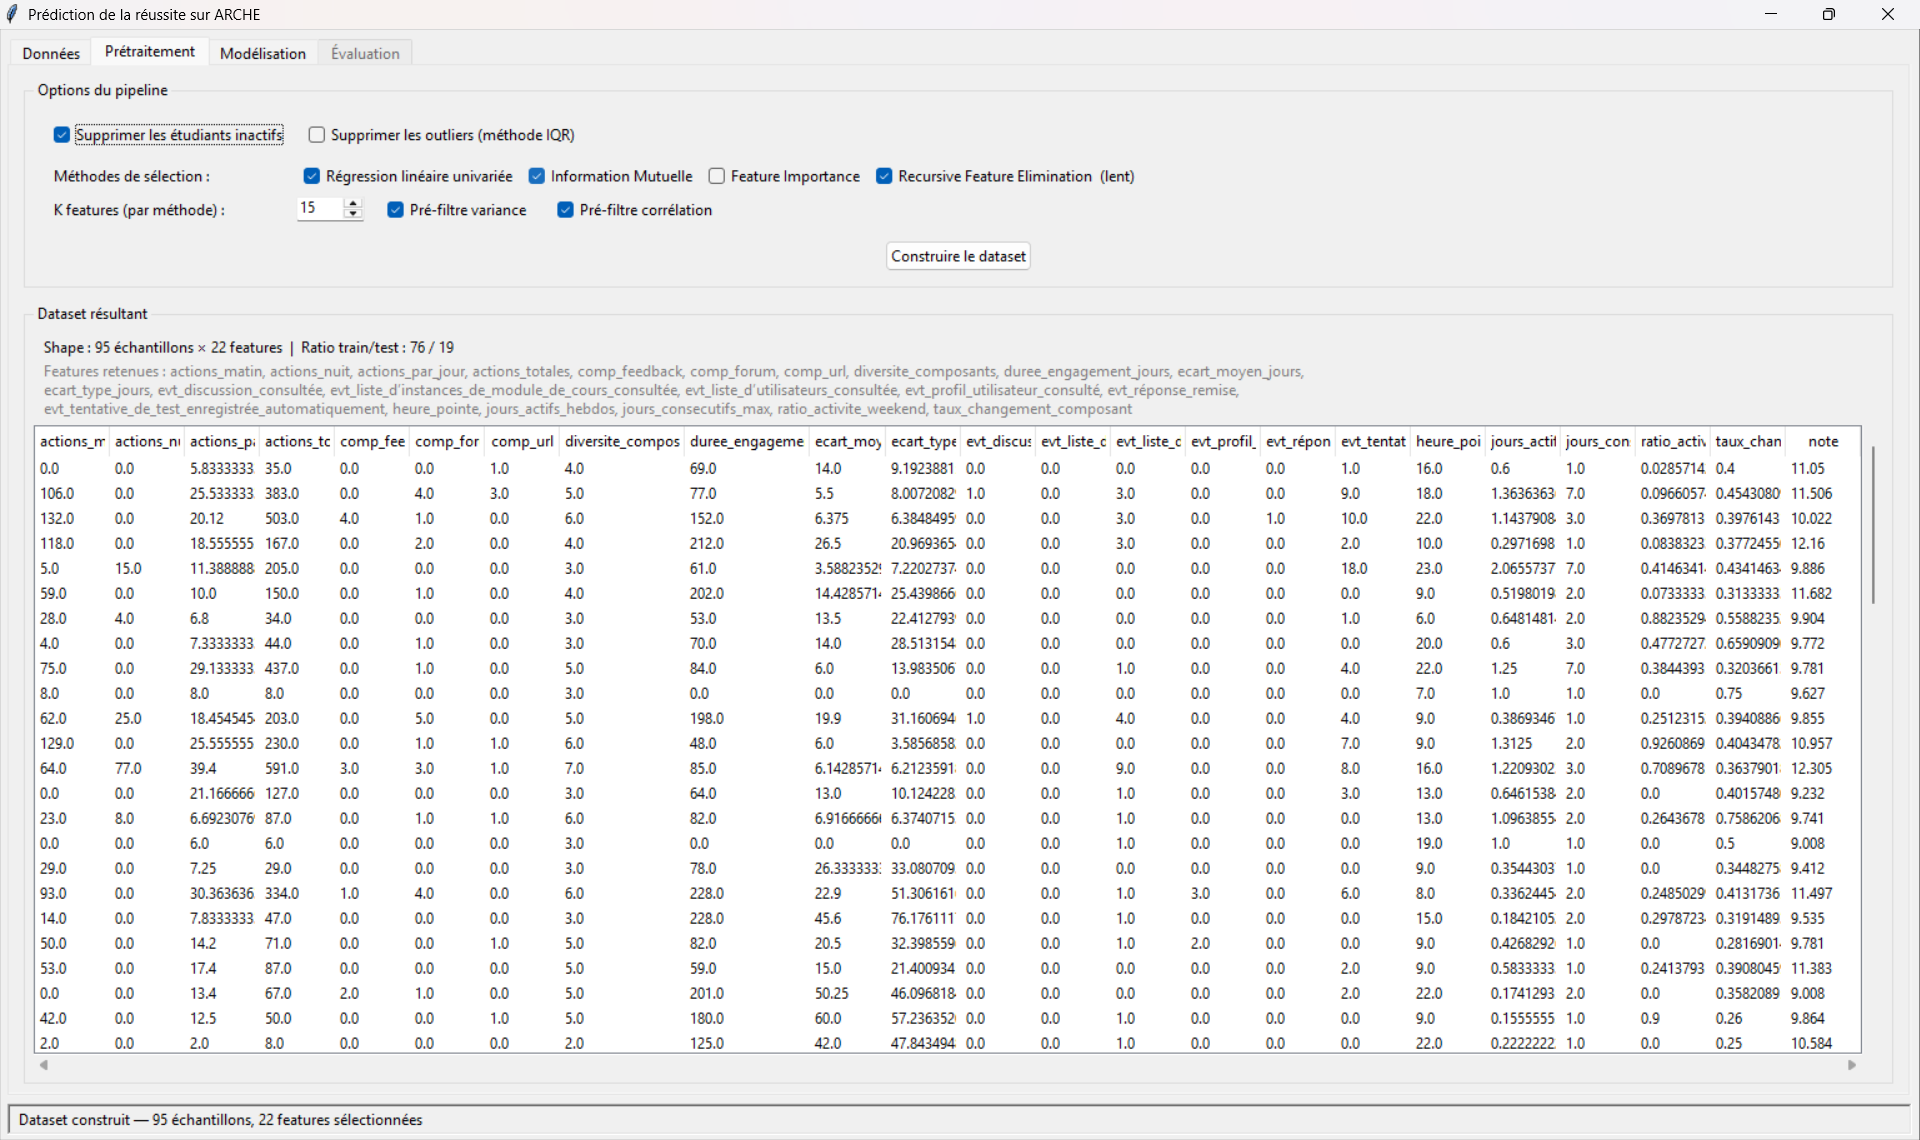
\includegraphics[width=0.92\textwidth]{../pictures/onglet2.png}
  \caption{Onglet \textit{Prétraitement} : Configuration du pipeline et dataset résultant}
\end{figure}


\begin{analysebox}{Variables sélectionnées}
D'après la session illustrée dans l'onglet Prétraitement, les 22 variables retenues incluent notamment : \texttt{actions\_matin}, \texttt{actions\_nuit}, \texttt{actions\_totales}, plusieurs colonnes \texttt{comp\_*}, \texttt{diversite\_composants}, \texttt{diversite\_contextes}, \texttt{duree\_engagement\_jours}, \texttt{jours\_actifs}, \texttt{jours\_consecutifs\_max}, \texttt{nombre\_sessions}, \texttt{ratio\_activite\_weekend}, etc.
\end{analysebox}

% ============================================================
\chapter{Modélisation}
% ============================================================

\section{Standardisation des données}

Avant l'entraînement de tout modèle, les variables sont standardisées à l'aide d'un \textbf{\texttt{RobustScaler}} :

\begin{equation}
  X_{\text{scaled}} = \frac{X - \mathrm{médiane}(X)}{\mathrm{IQR}(X)}
\end{equation}

Le \texttt{RobustScaler} a été préféré au \texttt{StandardScaler} car les données de logs présentent de fortes disparités.
La médiane et l'écart interquartile (IQR) sont robustes aux valeurs extrêmes, contrairement à la moyenne et à l'écart-type.

Le scaler est entraîné uniquement sur les données d'entraînement puis appliqué aux données de test, pour éviter toute fuite d'information (\textit{data leakage}).

\section{Modèle 1 : Régression Linéaire Multiple (RLM)}

La régression linéaire multiple modélise la note $y$ comme une combinaison linéaire des variables sélectionnées $x_1, \ldots, x_p$ :

\begin{equation}
  \hat{y} = \beta_0 + \beta_1 x_1 + \beta_2 x_2 + \cdots + \beta_p x_p
\end{equation}

Les coefficients $\beta_i$ sont estimés par la méthode des \textbf{moindres carrés ordinaires} (MCO) :

\begin{equation}
  \hat{\boldsymbol{\beta}}
  = \arg\min_{\boldsymbol{\beta}} \sum_{i=1}^n (y_i - \hat{y}_i)^2
  = (\mathbf{X}^\top \mathbf{X})^{-1} \mathbf{X}^\top \mathbf{y}
\end{equation}

Ce modèle suppose notamment la linéarité de la relation, la normalité des résidus (vérifiable via le test de Shapiro-Wilk) et l'absence de multicolinéarité, partiellement traitée par le pré-filtrage en amont.

\section{Modèle 2 : Random Forest (Forêt Aléatoire)}

La forêt aléatoire agrège les prédictions de $B$ arbres de décision :

\begin{equation}
  \hat{y}_{\text{RF}} = \frac{1}{B} \sum_{b=1}^{B} T_b(\mathbf{x})
\end{equation}

\begin{center}
\begin{tabular}{lll}
\toprule
\textbf{Paramètre} & \textbf{Valeur} & \textbf{Rôle}\\
\midrule
\texttt{n\_estimators}       & 200           & Nombre d'arbres\\
\texttt{max\_depth}          & 10            & Profondeur maximale\\
\texttt{max\_features}       & \texttt{sqrt} & Variables candidates par noeud\\
\texttt{min\_samples\_split} & 5             & Min. d'échantillons pour diviser\\
\texttt{bootstrap}           & False         & Sans remise (petit jeu de données)\\
\texttt{criterion}           & \texttt{friedman\_mse} & Critère de division\\
\bottomrule
\end{tabular}
\end{center}

\section{Modèle 3 : Gradient Boosting}

Le Gradient Boosting construit les arbres séquentiellement,
chacun corrigeant les erreurs du précédent :

\begin{equation}
  \hat{y}^{(m)} = \hat{y}^{(m-1)} + \eta \cdot T_m(\mathbf{x})
\end{equation}

où $\eta$ est le taux d'apprentissage et $T_m$ le $m$-ième arbre résiduel.

\begin{center}
\begin{tabular}{lll}
\toprule
\textbf{Paramètre} & \textbf{Valeur} & \textbf{Rôle}\\
\midrule
\texttt{n\_estimators}  & 100   & Nombre d'itérations (arbres)\\
\texttt{learning\_rate} & 0,1   & Taux d'apprentissage\\
\texttt{max\_depth}     & 3     & Arbres peu profonds\\
\texttt{subsample}      & 0,8   & Sous-échantillonnage stochastique\\
\bottomrule
\end{tabular}
\end{center}

% ============================================================
\chapter{Évaluation et comparaison des modèles}
% ============================================================

\section{Métriques de performance}

Trois métriques principales ont été calculées sur les données de test (19 observations) :

\begin{description}
  \item[$R^2$ (coefficient de détermination)]
    Proportion de la variance de la note expliquée par le modèle.
    Un $R^2 = 1$ correspond à une prédiction parfaite ;
    un $R^2 = 0$ revient à prédire la moyenne ;
    un $R^2 < 0$ signifie que le modèle est moins bon que la prédiction naïve.
  \item[RMSE (\textit{Root Mean Squared Error})]
    Erreur quadratique moyenne, exprimée en points de note.
    Pénalise davantage les erreurs importantes.
  \item[MAE (\textit{Mean Absolute Error})]
    Erreur absolue moyenne, exprimée en points de note.
    Plus robuste aux erreurs extrêmes.
\end{description}

\section{Résultats obtenus}

\begin{table}[H]
\centering
\caption{Comparaison des performances sur les données de test (19 observations)}
\begin{tabular}{lrrr}
\toprule
\textbf{Modèle} & \textbf{$R^2$} & \textbf{RMSE} & \textbf{MAE}\\
\midrule
Régression Linéaire & $-0{,}4260$ & $1{,}2073$ & $0{,}9431$\\
Random Forest       & $+0{,}1262$ & $0{,}9451$ & $0{,}7828$\\
Gradient Boosting   & $-0{,}2601$ & $1{,}1349$ & $0{,}8710$\\
\bottomrule
\end{tabular}
\end{table}

\section{Visualisations}

\begin{figure}[H]
  \centering
  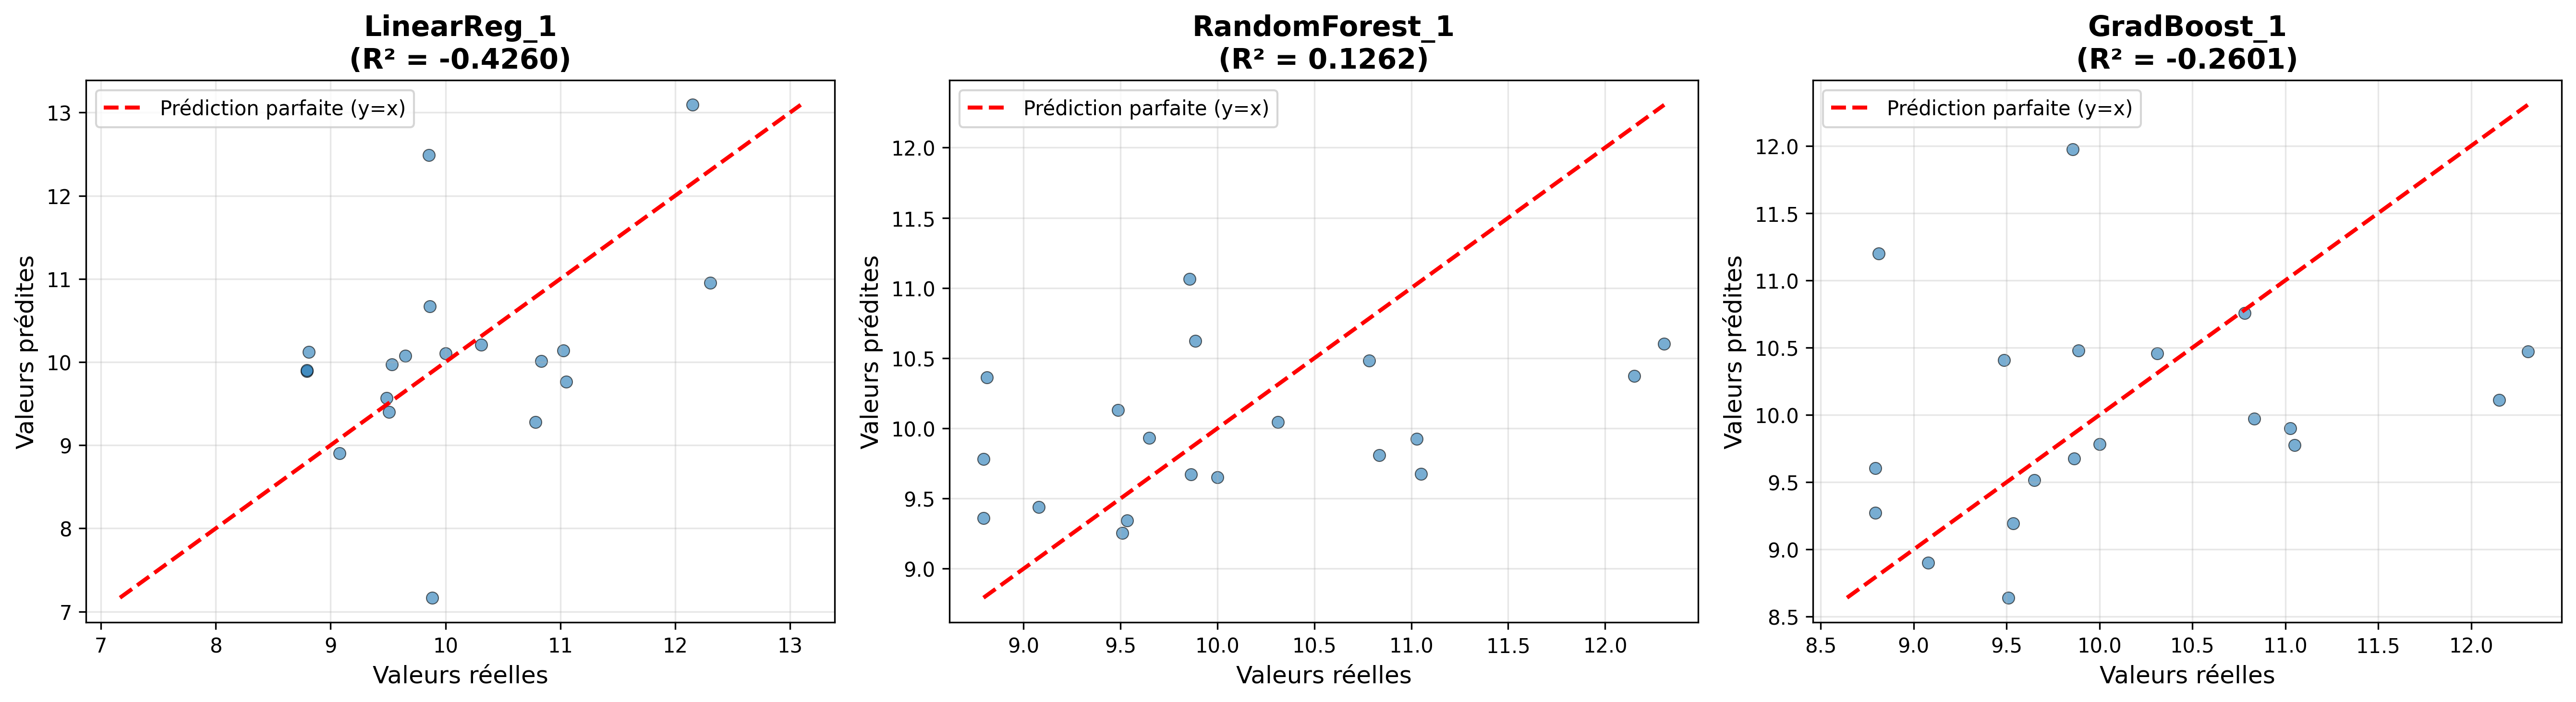
\includegraphics[width=\textwidth]{../output/predictions_comparison.png}
  \caption{Prédictions vs valeurs réelles pour les trois modèles}
\end{figure}

\begin{figure}[H]
  \centering
  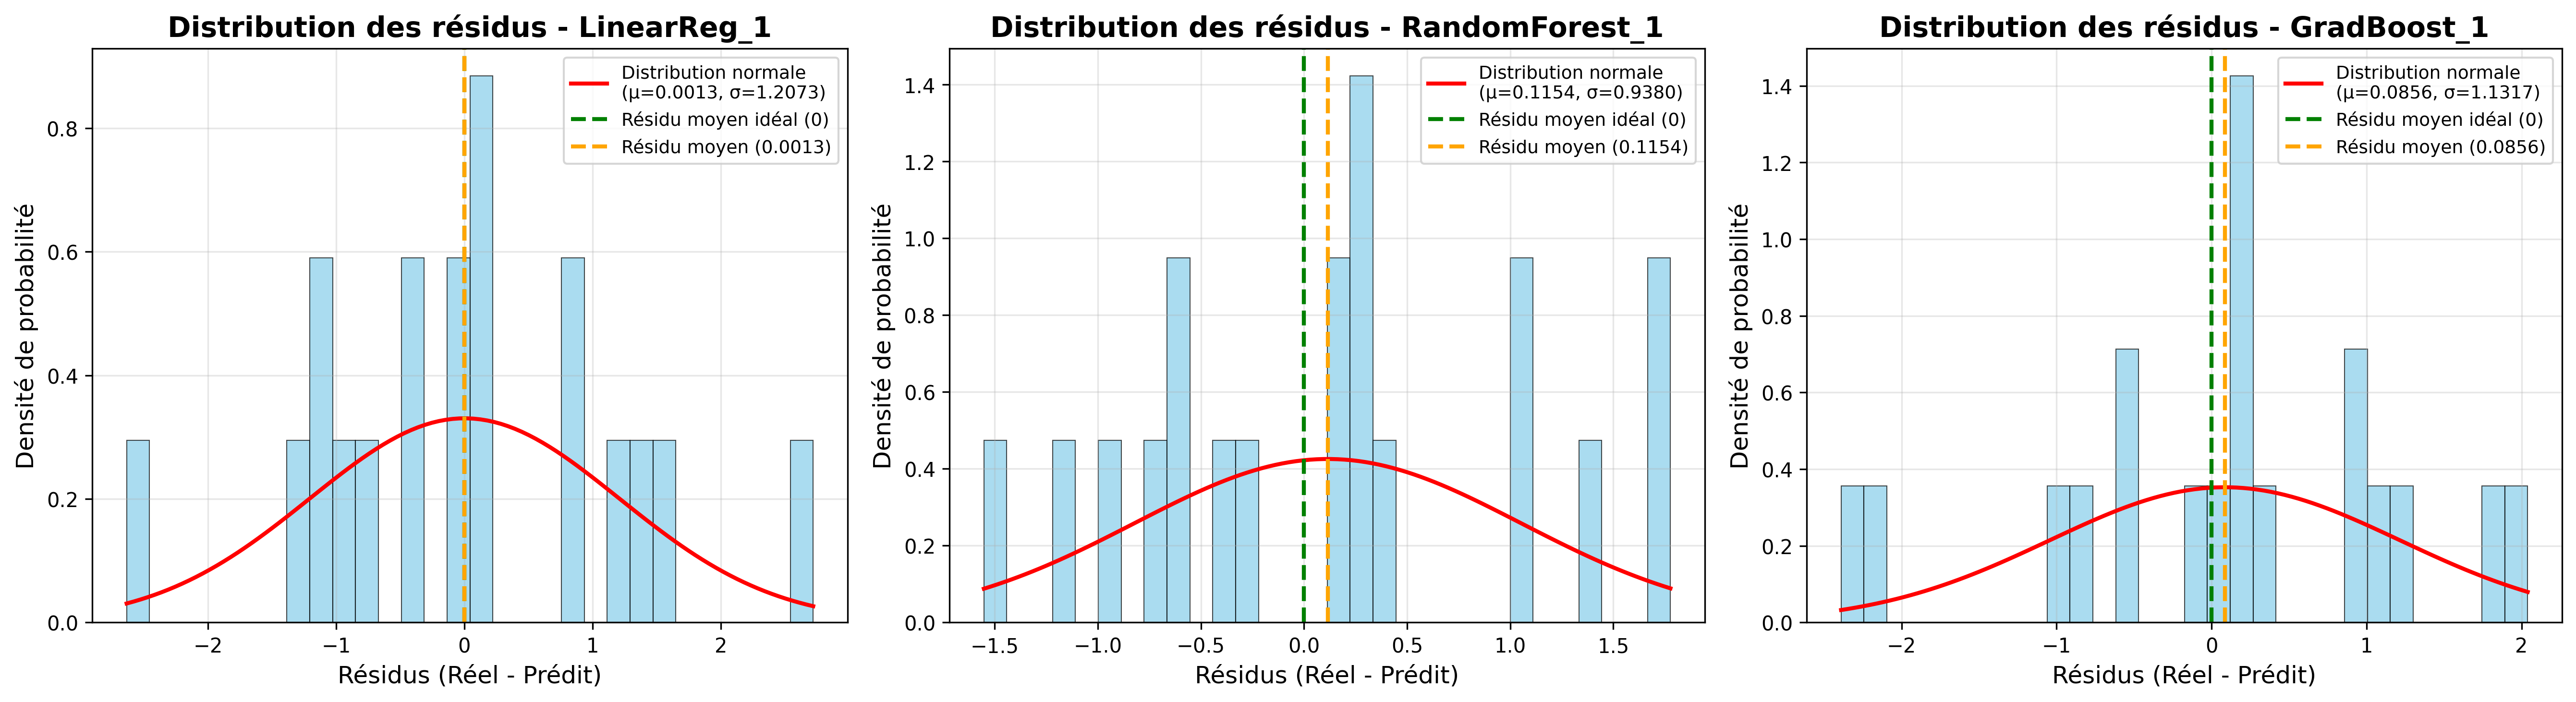
\includegraphics[width=\textwidth]{../output/residuals_comparison.png}
  \caption{Distribution des résidus pour les trois modèles}
\end{figure}

\begin{figure}[H]
  \centering
  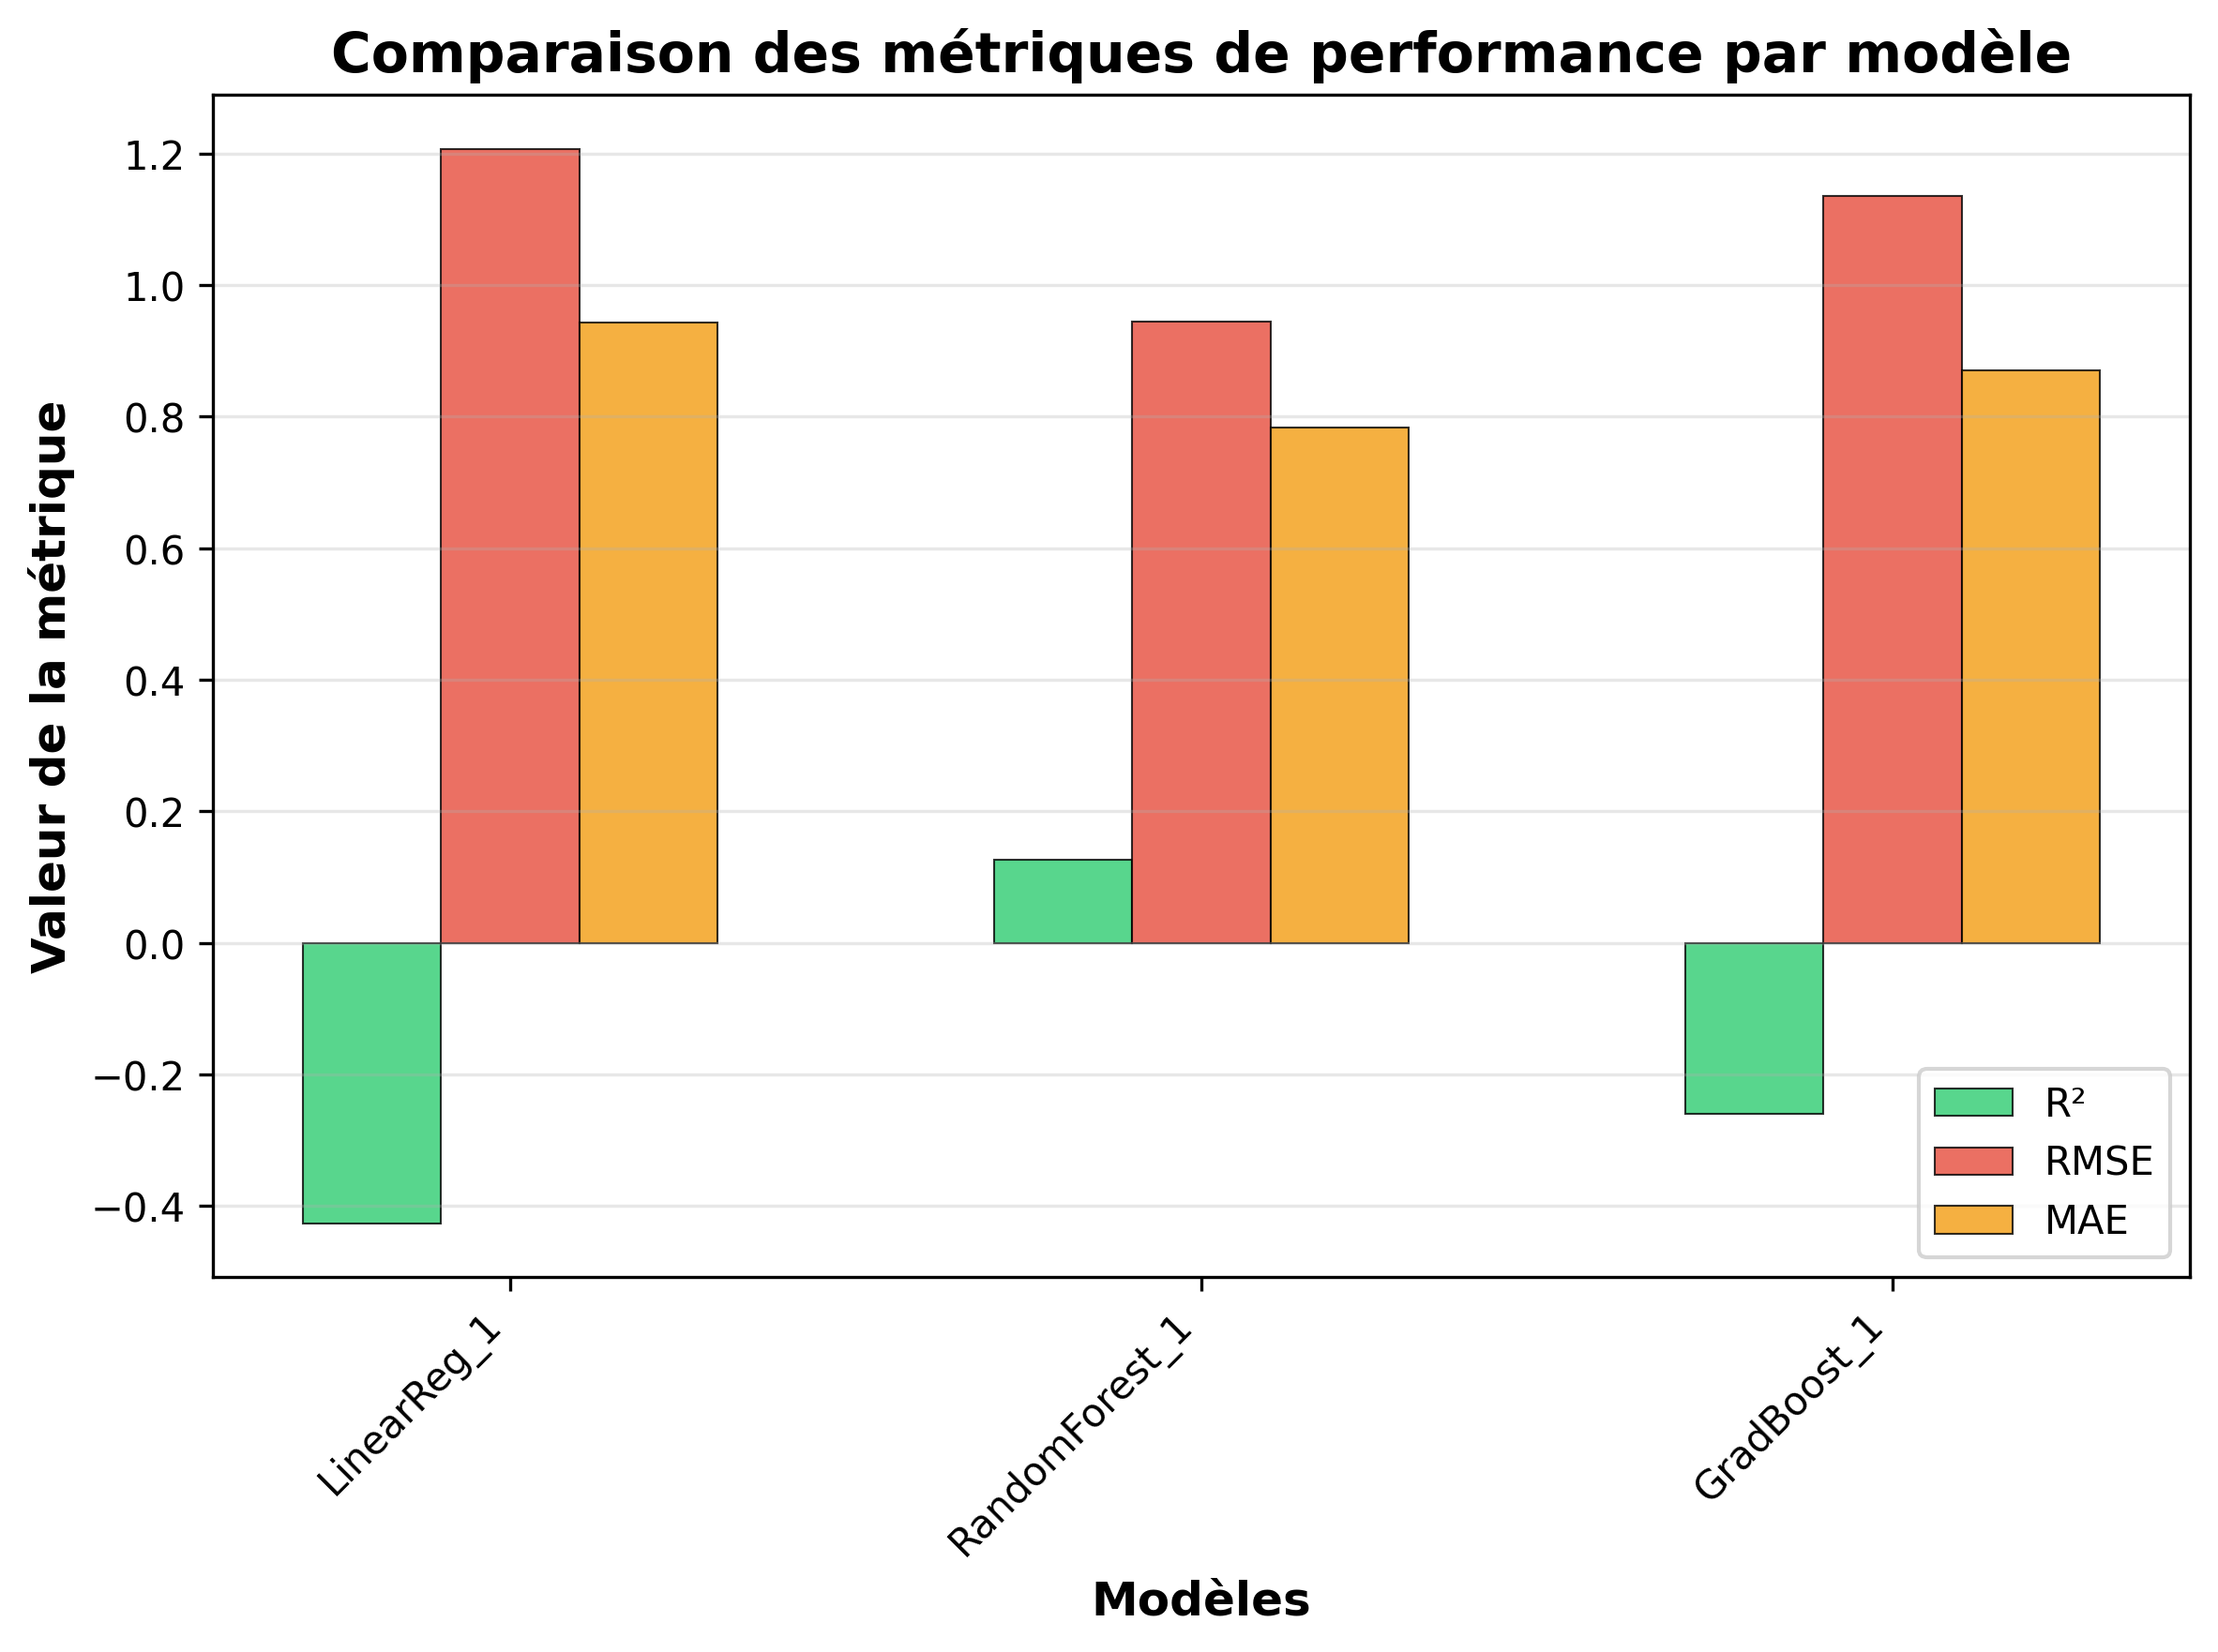
\includegraphics[width=0.55\textwidth]{../output/metrics_comparison.png}
  \caption{Comparaison des métriques par modèle}
\end{figure}

\section{Analyse des résultats}

\begin{warningbox}[Résultats très limités]
Les résultats sont clairement insuffisants pour constituer un modèle prédictif utilisable.
\begin{itemize}
  \item \textbf{Régression linéaire ($R^2 = -0{,}43$) :} le modèle prédit moins bien
        que la simple moyenne des notes, signe d'un problème de linéarité ou de sur-apprentissage.
  \item \textbf{Gradient Boosting ($R^2 = -0{,}26$) :} même constat.
  \item \textbf{Random Forest ($R^2 = +0{,}13$) :} seul modèle légèrement positif,
        mais avec un RMSE de 0,95 point, la prédiction reste très imprécise.
\end{itemize}
\end{warningbox}

La meilleure performance du Random Forest s'explique par sa capacité à modéliser des relations non linéaires et des interactions entre variables, sans nécessiter les hypothèses strictes de la régression linéaire.
Cependant, avec seulement 95 observations et une vingtaine de variables, le risque de sur-apprentissage est élevé.

Les graphiques de prédictions vs valeurs réelles confirment ce diagnostic : les points sont largement dispersés autour de la diagonale, sans tendance claire.

% ============================================================
\chapter{Discussion, limites et perspectives}
% ============================================================

\section{Pourquoi ces résultats sont-ils décevants ?}

\subsection{Taille insuffisante du jeu de données}

Avec \textbf{95~étudiants} pour une vingtaine de variables,
le jeu de données est très petit au regard des standards du Machine Learning. La règle empirique recommande au minimum 10 à 20 observations par variable explicative. Ici, le ratio est à peine de 4 à 5, ce qui favorise le sur-apprentissage (diminuer le nombre de variables sélectionnées n'améliore toutefois pas les scores).

\subsection{Questionnement sur la pertinence des variables}

Les features extraites des logs capturent une présence \textit{quantitative} sur la plateforme, mais pas la qualité du travail fourni, ni les facteurs extérieurs à la plateforme.

\vspace{0.3cm}
\noindent Or, la réussite scolaire est un phénomène multifactoriel :
\begin{itemize}
  \item qualité du travail personnel hors ligne ;
  \item capacités cognitives individuelles ;
  \item contexte socio-économique ;
  \item présence en cours, participation aux TD/TP ;
  \item motivation, état émotionnel, santé.
\end{itemize}

Un étudiant peu actif sur ARCHE peut très bien réussir en travaillant intensivement sur ses supports papier. Les traces numériques ne capturent qu'une infime partie des facteurs explicatifs.

\subsection{Absence d'optimisation des hyperparamètres}

Par manque de temps, la recherche d'hyperparamètres optimaux
(via \texttt{GridSearchCV} ou \texttt{RandomizedSearchCV}) n'a pas été réalisée. La validation croisée (\textit{cross-validation}), qui permettrait une estimation plus robuste des performances, n'a pas non plus été mise en oeuvre.

\subsection{Contraintes techniques}

L'interdiction des notebooks Jupyter a complexifié la phase d'exploration et d'itération rapide. Les notebooks sont l'outil standard pour le travail exploratoire en data science (CRISP-DM), permettant de visualiser rapidement les données et d'affiner le feature engineering de façon interactive.

\section{Une classification aurait peut-être été plus adaptée}

Compte tenu des données disponibles et de l'objectif pratique du projet (identifier les étudiants en difficulté), une approche de \textbf{classification} aurait été plus pertinente qu'une régression.

L'idée serait de transformer la variable cible :
\begin{equation}
  \mathrm{classe} = \begin{cases}
    \text{À risque}    & \text{si } \mathrm{note} < 10 \\
    \text{En réussite} & \text{si } \mathrm{note} \geq 10
  \end{cases}
\end{equation}

\noindent Cette approche présente plusieurs avantages :
\begin{itemize}
  \item une cible binaire est généralement plus facile à prédire
        qu'une valeur continue sur 20 ;
  \item les métriques de classification (précision, rappel, F1-score, AUC-ROC) sont plus interprétables dans un contexte pédagogique ;
  \item l'asymétrie des erreurs peut être modélisée explicitement : une fausse alarme est moins grave qu'un étudiant à risque non détecté.
\end{itemize}

\noindent Cette évolution est envisagée pour la soutenance orale.

\section{Pistes d'amélioration}

\begin{enumerate}
  \item \textbf{Passer à la classification} avec \texttt{SVC} (petit dataset), \texttt{RandomForestClassifier} ou \texttt{GradientBoostingClassifier}.

  \item \textbf{Enrichir les données} en croisant avec d'autres sources (assiduité en présentiel, résultats intermédiaires, profil étudiant) pour obtenir des variables plus prédictives.

  \item \textbf{Optimiser les hyperparamètres} via une recherche randomisée avec validation croisée stratifiée.

  \item \textbf{Approfondir le feature engineering :}
        \begin{itemize}
          \item tendance temporelle (l'activité augmente-t-elle avant les examens ?) ;
          \item ratio soumissions / consultations (engagement actif vs passif).
        \end{itemize}

  \item \textbf{Augmenter le jeu de données} en agrégeant plusieurs promotions ou plusieurs cours pour atteindre une taille d'échantillon suffisante.
\end{enumerate}

% ============================================================
% Conclusion
% ============================================================
\chapter*{Conclusion}
\addcontentsline{toc}{chapter}{Conclusion}

Ce projet a permis de mettre en oeuvre un pipeline complet de data science sur un jeu de données réel, du chargement jusqu'à la comparaison de modèles, dans le respect des contraintes imposées (interface Tkinter, sans notebook Jupyter).

Les résultats obtenus sont frustrants et décevants d'un point de vue prédictif : aucun des trois modèles testés ne parvient à prédire la note d'un étudiant de façon fiable. Cela tient à la faible taille du jeu de données, à la nature limitée des informations disponibles dans les logs, et à l'absence d'optimisation systématique des hyperparamètres.

Ces constats illustrent une réalité fréquente en data science : disposer d'un pipeline technique robuste ne suffit pas. La \textbf{qualité et la pertinence des données} sont le facteur déterminant de la performance d'un modèle prédictif.

La piste la plus prometteuse pour la suite serait de reformuler le problème comme une tâche de \textbf{classification} (étudiant à risque vs en réussite), plus robuste statistiquement et plus actionnable pédagogiquement.

\end{document}
